%% abtex2-modelo-artigo.tex, v-1.8 laurocesar
%% Copyright 2012-2013 by abnTeX2 group at http://abntex2.googlecode.com/ 
%%
%% This work may be distributed and/or modified under the
%% conditions of the LaTeX Project Public License, either version 1.3
%% of this license or (at your option) any later version.
%% The latest version of this license is in
%%   http://www.latex-project.org/lppl.txt
%% and version 1.3 or later is part of all distributions of LaTeX
%% version 2005/12/01 or later.
%%
%% This work has the LPPL maintenance status `maintained'.
%% 
%% The Current Maintainer of this work is the abnTeX2 team, led
%% by Lauro César Araujo. Further information are available on 
%% http://abntex2.googlecode.com/
%%
%% This work consists of the files abntex2-modelo-artigo.tex and
%% abntex2-modelo-references.bib
%%

% ------------------------------------------------------------------------
% ------------------------------------------------------------------------
% abnTeX2: Modelo de Artigo Acadêmico em conformidade com
% ABNT NBR 6022:2003: Informação e documentação - Artigo em publicação 
% periódica científica impressa - Apresentação
% ------------------------------------------------------------------------
% ------------------------------------------------------------------------

\documentclass[
	% -- opções da classe memoir --
	article,			% indica que é um artigo acadêmico
	11pt,				% tamanho da fonte
	oneside,			% para impressão apenas no verso. Oposto a twoside
	a4paper,			% tamanho do papel. 
	% -- opções da classe abntex2 --
	%chapter=TITLE,		% títulos de capítulos convertidos em letras maiúsculas
	%section=TITLE,		% títulos de seções convertidos em letras maiúsculas
	%subsection=TITLE,	% títulos de subseções convertidos em letras maiúsculas
	%subsubsection=TITLE % títulos de subsubseções convertidos em letras maiúsculas
	% -- opções do pacote babel --
	english,			% idioma adicional para hifenização
	brazil,				% o último idioma é o principal do documento
	]{abntex2}


% ---
% PACOTES
% ---

% ---
% Pacotes fundamentais 
% ---
\usepackage{cmap}				% Mapear caracteres especiais no PDF
\usepackage{lmodern}			% Usa a fonte Latin Modern
\usepackage[T1]{fontenc}		% Selecao de codigos de fonte.
\usepackage[utf8]{inputenc}		% Codificacao do documento (conversão automática dos acentos)
\usepackage{indentfirst}		% Indenta o primeiro parágrafo de cada seção.
\usepackage{nomencl} 			% Lista de simbolos
\usepackage{color}				% Controle das cores
\usepackage{graphicx}			% Inclusão de gráficos
\usepackage{url}
% ---
		
% ---
% Pacotes adicionais, usados apenas no âmbito do Modelo Canônico do abnteX2
% ---
\usepackage{lipsum}				% para geração de dummy text
% ---
		
% ---
% Pacotes de citações
% ---
\usepackage[brazilian,hyperpageref]{backref}	 % Paginas com as citações na bibl
\usepackage[alf]{abntex2cite}	% Citações padrão ABNT
% ---

% ---
% Configurações do pacote backref
% Usado sem a opção hyperpageref de backref
\renewcommand{\backrefpagesname}{Citado na(s) página(s):~}
% Texto padrão antes do número das páginas
\renewcommand{\backref}{}
% Define os textos da citação
\renewcommand*{\backrefalt}[4]{
	\ifcase #1 %
		Nenhuma citação no texto.%
	\or
		Citado na página #2.%
	\else
		Citado #1 vezes nas páginas #2.%
	\fi}%
% ---

% ---
% Informações de dados para CAPA e FOLHA DE ROSTO
% ---
\titulo{\emph{Cymbopognon nardus} - Citronela}
\autor{Chrystian de Sousa Guth\thanks{csguth@gmail.com}}
\local{Florianópolis}
\data{Florianópolis, Outubro de 2013 \par
	Universidade Federal de Santa Catarina
	\par 
	Centro de Ciências da Saúde
	\par 
	Departamento de Enfermagem}

% ---

% ---
% Configurações de aparência do PDF final

% alterando o aspecto da cor azul
\definecolor{blue}{RGB}{41,5,195}

% informações do PDF
\makeatletter
\hypersetup{
     	%pagebackref=true,
		pdftitle={\@title}, 
		pdfauthor={\@author},
    	pdfsubject={Modelo de artigo científico com abnTeX2},
	    pdfcreator={LaTeX with abnTeX2},
		pdfkeywords={abnt}{latex}{abntex}{abntex2}{atigo científico}, 
		colorlinks=true,       		% false: boxed links; true: colored links
    	linkcolor=blue,          	% color of internal links
    	citecolor=blue,        		% color of links to bibliography
    	filecolor=magenta,      		% color of file links
		urlcolor=blue,
		bookmarksdepth=4
}
\makeatother
% --- 

% ---
% compila o indice
% ---
\makeindex
% ---

% ---
% Altera as margens padrões
% ---
\setlrmarginsandblock{4cm}{4cm}{*}
\setulmarginsandblock{4cm}{4cm}{*}
\checkandfixthelayout
% ---

% --- 
% Espaçamentos entre linhas e parágrafos 
% --- 

% O tamanho do parágrafo é dado por:
\setlength{\parindent}{1.3cm}

% Controle do espaçamento entre um parágrafo e outro:
\setlength{\parskip}{0.2cm}  % tente também \onelineskip

% Espaçamento simples
\SingleSpacing

% ----
% Início do documento
% ----
\begin{document}

% Retira espaço extra obsoleto entre as frases.
\frenchspacing 

% ----------------------------------------------------------
% ELEMENTOS PRÉ-TEXTUAIS
% ----------------------------------------------------------

% página de titulo
\maketitle

% ----------------------------------------------------------
% ELEMENTOS TEXTUAIS
% ----------------------------------------------------------
\textual

% ----------------------------------------------------------
% Introdução
% ----------------------------------------------------------
\section*{Introdução}
\addcontentsline{toc}{section}{Introdução}


A natureza proporciona ao homem uma infinidade de plantas com valores medicinais, e a sua utilização como medicamento é tão antiga quanto o aparecimento da própria raça humana \cite{sossae2013}. As plantas, pelas suas propriedades terapeuticas ou tóxicas, adquiriram fundamental importância na manutenção da vida animal, sendo utilizadas na nutrição, tratamento de enfermidades ou mesmo como ``arma'' contra algum tipo de agente prejudicial.

Entre uma das diversas espécies de plantas que podem ser utilizadas com objetivo medicinal, podemos citar a \emph{Cymbopognon}, em especial o gênero \emph{Cymbopognon nardus}, conhecida popularmente como Citronela \cite{fao2013}.

Este trabalho tem por objetivo, apresentar informações relevantes sobre a citronela e seu uso na prática medicinal, desde sua classificação científica, região de origem e as formas mais comuns de manuseio desta planta, que é bastante conhecida popular e cientificamente.

\section{\emph{Cymbopognon nardus}}

A \emph{Cymbopognon nardus}, ou \emph{Cymbopogon afronardus Stapf.}, também conhecida como Citronela Falsa (Zaire), Capim Citronela (Taiwan), Capim Citronela Azul (Kenya) e outros \footnote{False citronella (Zaire), citronella grass (Taiwan), blue citronella grass (Kenya), Tussocky Guinea grass (Uganda), naid grass (India).}, ou apenas, Citronela, é uma planta perene de origem africana, de onde é extraído um óleo essencial (Figura \ref{fig:oleo_essencial}), geralmente utilizado como repelente de insetos. Com folhas compridas, finas e pontudas, seus arbustos podem chegar à altura de 2 metros, e visualmente é bem parecida com um outro gênero de \emph{Cymbopognon}, o \emph{Cymbopognon citratus}, ou Capim-Limão, como pode ser observado na Figura \ref{fig:capim_limao_citronela}.

\begin{figure}[tb]
	\begin{center}
		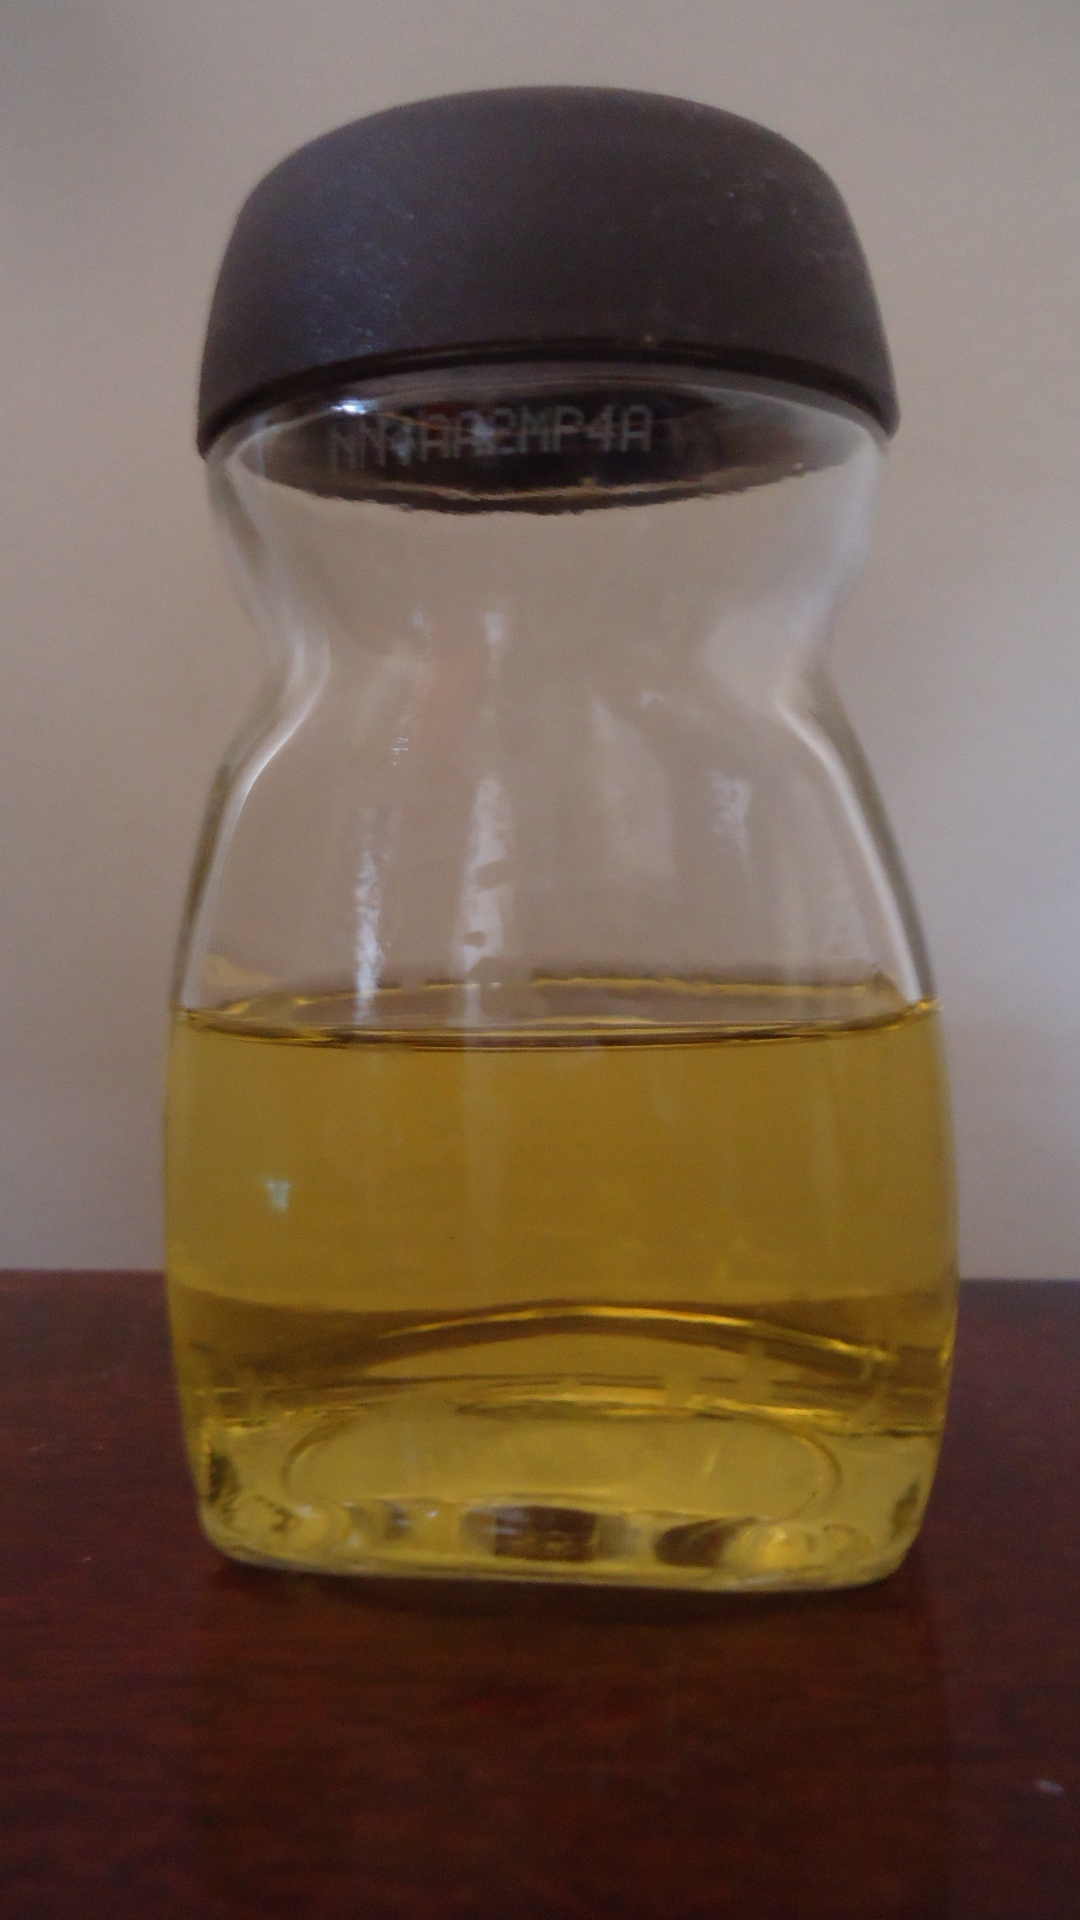
\includegraphics[scale=0.1]{imgs/oleo_essencial.jpg} 
		\caption{Recipiente de vidro armazenando óleo essencial extraído da \emph{Cymbopognon citratus}}
		\label{fig:oleo_essencial}
	\end{center}
\end{figure}

\begin{figure}[tb]
	\begin{center}
		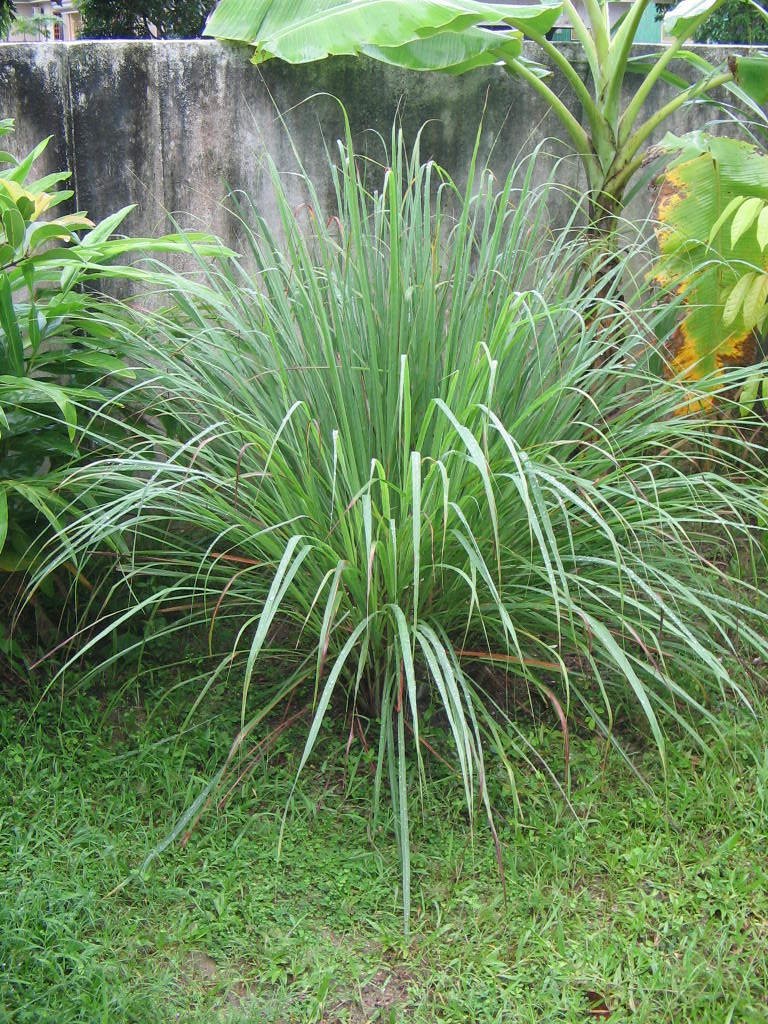
\includegraphics[scale=0.15]{imgs/capim_limao.JPG} \quad 
		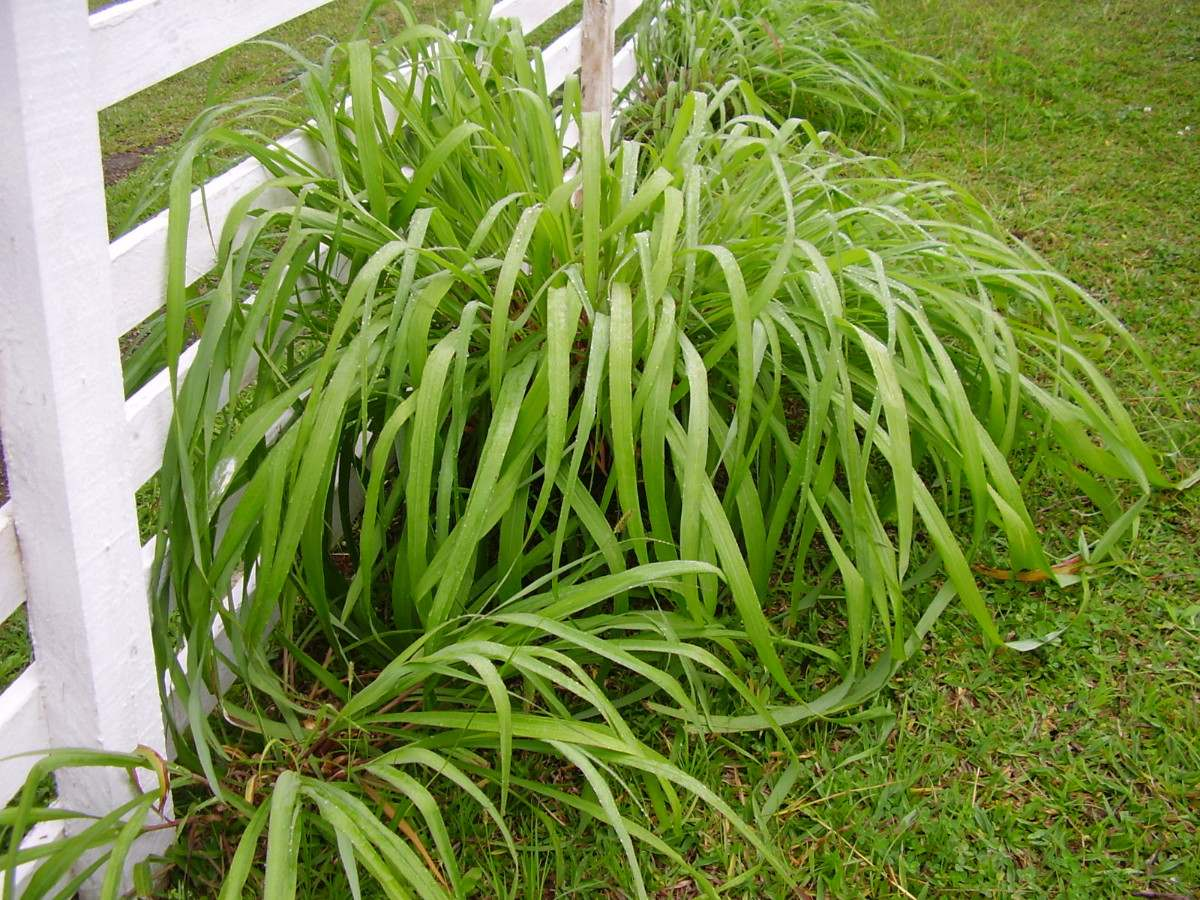
\includegraphics[scale=0.15]{imgs/citronela.jpg} 
		\caption{À esquerda, um exemplar de \emph{Cymbopognon citratus}, ou Capim-Limão e à direita, a \emph{Cymbopognon nardus}, popularmente conhecida como Citronela.}
		\label{fig:capim_limao_citronela}
	\end{center}
\end{figure}



\subsection{Classificação Científica}

\begin{itemize}

	\item \textbf{Reino:}	\emph{Plantae}

	\item \textbf{Divisão:} \emph{Magnoliophyta}

	\item \textbf{Classe:}	\emph{Liliopsida}

	\item \textbf{Ordem:}	\emph{Poales}

	\item \textbf{Família:}	 \emph{Poaceae}

	\item \textbf{Género:}	\emph{Cymbopogon Spreng.}

	\item \textbf{Espécie:}	 \emph{C. nardus.}

\end{itemize}

\subsection{Óleo Essencial de Citronela}
O óleo de citronela, é um óleo extraído das folhas e caule da citronela. Rico em geraniol, citronelol e citronelal, é utilizado na fabricação de velas, cremes e loções. O uso mais comum do óleo de citronela é como biopesticida de ação não tóxica. O estudo de \citeauthor{pattnaik95} de \citeyear{pattnaik95}, mostra também que o óleo de citronela possui propriedades antifúngicas.

Este óleo essencial pode ser extraído de forma caseira, porém não é muito simples. As folhas e caule são colocadas em uma panela de pressão com água, assim, o vapor liberado, contém também, óleo essencial. De forma industrial, as folhas, acomodadas em um recipiente, recebem vapor de água constantemente. Por condensação, o óleo pode ser separado da água, e assim, armazenado.

\subsubsection{Principais componentes químicos do óleo essencial de Citronela}
O Geraniol ($C_{10}H_{18}O$), citado anteriormente, é um dos elementos contidos no óleo de Citronela. Ele possui um odor semelhante ao de rosas, proporcionando sua aplicação na perfumaria. O Geraniol apresenta também, atividade antibacteriana contra \emph{Salmonella typhimurium}, como mostra o estudo \cite{kim1995}. Outros estudos evidenciam o Geraniol como um efetivo repelente de insetos \cite{barnard2004}, porém, pode atrair abelhas, já que elas o produzem para marcar as flores de onde estão realizando a extração de néctar.

Outro componente importante encontrado no óleo essencial de citronela é o Citronelol ($C_{10}H_{20}O$). Assim como o Geraniol, o Citronelol é utilizado em perfumes e também atua como repelente de insetos. Na perfumaria, esta substância deve ser evitada por pessoas sensíveis, pois dependendo da quantidade, pode causar reações alérgicas.

O Citronelal ($C_{10}H_{18}O$), outro componente importante do óleo. Este é o principal responsável pelo odor de limão acentuado apresentado no óleo de citronela. O Citronelal apresenta também propriedades repelentes, com grande eficácia contra mosquitos \cite{kim2005}, além também, das suas propriedades anti-fúngicas \cite{nakahara2003}.

\subsubsection{Utilização do óleo de citronela no controle do carrapato de bovinos}

As perdas econômicas causadas por parasitas externos em rebanhos bovinos no Brasil, superam a cifra de 2 bilhões de dólares ao ano. Cerca de 75\% dessa perda, é atribuida ao carrapato, e os outros 25\% a outros parasitas, como a mosca-dos-chifres, o berne, miíases, mosca-dos-estábulos, etc \cite{grisi2002}. 

Geralmente, o controle de parasitoses é realizado utilizando produtos químicos, que acabam causando danos, não só ao bovino, mas também ao homem, que consome a carne e outros produtos de origem animal \cite{chagas2003}.

Em \citeyear{clair2008}, \citeauthor{clair2008} realizaram um experimento em fêmeas de bovinos da raça Holandesa, naturalmente infestados, pertencentes ao Laboratório de Bovinocultura de Leite, da Universidade Federal de Santa Maria (UFSM). O óleo utilizado é originário do Rio Grande do Sul, e os testes foram realizados em diferentes concentrações, com um rendimento de aproximadamente 0.7\%. A partir deste estudo, comprova-se que o óleo de citronela, além de ter uma boa eficácia contra a proliferação do carrapato bovino, também tem acão acaricida, apresentando uma eficiência de 50\% no controle das larvas, utilizando concentrações de 6,1 e 4,1\%.

\section{Conclusão}

A arte milenar de se utilizar plantas com fins medicinais está em constante aperfeiçoamento, e o avanço dos estudos em determinadas espécies possibilita à raça humana, uma melhor qualidade de vida. A Citronela, é uma das plantas medicinais que tem um papel muito importante na manutenção da vida, pois as substâncias encontradas em seu óleo essencial apresentam diversas utilizações, desde a aplicação na perfumaria, até sua utilização como repelente contra insetos. É comprovado também, que o óleo de citronela tem acão acaricida, impedindo a criação de larvas, e vem sendo utilizado no controle de carrapatos nos bovinos. A utilização do óleo de citronela nos bovinos tem baixa toxidade, e reduz os prejuízos causados por pestes nos rebanhos, que chegam a custar 2 bilhões de dólares por ano no Brasil.

% ]  				% FIM DE ARTIGO EM DUAS COLUNAS
% ---

% ----------------------------------------------------------
% Referências bibliográficas
% ----------------------------------------------------------
\bibliography{referencias}

% ----------------------------------------------------------
% Glossário
% ----------------------------------------------------------
%
% Há diversas soluções prontas para glossário em LaTeX. 
% Consulte o manual do abnTeX2 para obter sugestões.
%
%\glossary

% ----------------------------------------------------------
% Apêndices
% ----------------------------------------------------------

% ---
% Inicia os apêndices
% ---
%\begin{apendicesenv}
%
%% ----------------------------------------------------------
%\chapter{Nullam elementum urna vel imperdiet sodales elit ipsum pharetra ligula
%ac pretium ante justo a nulla curabitur tristique arcu eu metus}
%% ----------------------------------------------------------
%\lipsum[55-57]
%
%\end{apendicesenv}
% ---

% ----------------------------------------------------------
% Anexos
% ----------------------------------------------------------
%\cftinserthook{toc}{AAA}
% ---
% Inicia os anexos
% ---
%\anexos
%\begin{anexosenv}
%
%% ---
%\chapter{Cras non urna sed feugiat cum sociis natoque penatibus et magnis dis
%parturient montes nascetur ridiculus mus}
%% ---
%
%\lipsum[31]
%
%\end{anexosenv}

\end{document}
